В настоящее время большую популярность набирают онлайн продажи различных товаров
и услуг. Одним из таких направлений является доставка еды из кафе и ресторанов.
Пользователю предлагается выбрать понравившиеся блюда, оформить заказ и оплатить
его через интернет, используя только свой компьютер или телефон.

В апреле 2018 года компанией «Примнет» во Владивостоке был запущен проект "VLru Еда" \cite{VLruEda}.
На данный момент на сайте размещено более 100 компаний и около 8200 блюд. Каждый
день совершается большое количество заказов, но пользователям очень сложно сделать
выбор из такого объема товаров. Перед компанией стоит задача помочь клиенту в этом
нелегком вопросе. Для этого на всех этапах, от первого посещения сайта и до
оформления заказа, собирается информация о пользователе и действиях, которые он
совершил. С помощью этих данных решается большой спектр задач: какие интерфейсные
изменения необходимо внести, какого функционала не хватает для комфортного
использования сайта. и другие. Все это помогает пользователю быстрее находить интересующие
его блюда и совершить заказ.
\begin{figure}[H]
    \centering
    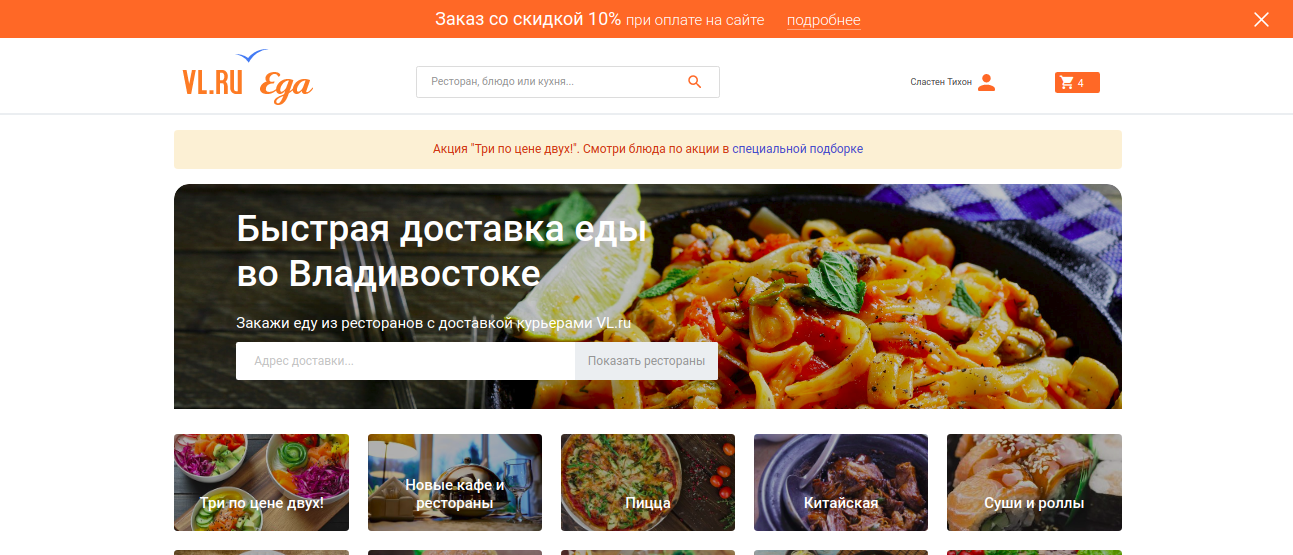
\includegraphics[scale=0.3]{images/main_page.png}
    \caption{Главная страница сайта "VLru Еда"}
\end{figure}

Увеличение количества продаж - это основная задача на протяжении всего жизненного
цикла любой компании. Область рекомендательных систем получила свое бурное развитие
около 20 лет назад. С помощью вышеуказанных систем появилась возможность выявления
интересов пользователя и, соответственно, предложения ему наиболее подходящих
товаров или услуг. Основываясь на положительном опыте в этой области таких крупных
компаний, как Netflix, Amazon и др., было принято решение реализовать рекомендательную
систему, которая могла бы предложить клиенту персонализированную подборку блюд на
сайте проекта "VLru Еда".
